
%----------------------------------------------------------------------------------------
% Lecture 4: Math AD-AS (Bridge from Lecture 3 figures to equations)
% Template: SimpleDarkBlue (based on user's slide_outline.tex)
% Figures expected in ./figureAD/ :
%   figAD0.jpg figAD1.jpg figAD2.jpg
%   figAS.jpg figAS0.jpg figAS1.jpg figAS2.jpg
%   figADAS.jpg figADAS1.jpg figADAS2.jpg figADAS3.jpg figADAS4.jpg
%----------------------------------------------------------------------------------------

\documentclass[aspectratio=169,xcolor=dvipsnames]{beamer}
\usetheme{SimpleDarkBlue}

\usepackage{hyperref}
\usepackage{graphicx}
\usepackage{booktabs}
\usepackage{appendixnumberbeamer}
\usepackage{amsmath}
\usepackage{iftex}

% --- Font handling (compile anywhere) ---
\ifPDFTeX
  \usepackage[T1]{fontenc}
  \usepackage{lmodern}
  \usepackage{microtype}
\else
  \usepackage{fontspec}
  \usepackage{luatexja}
  \setmainfont{Alegreya Sans Light}[
    ItalicFont={* Italic},
    BoldFont={Alegreya Sans Medium},
    BoldItalicFont={Alegreya Sans Medium Italic}]
  \setsansfont{Alegreya Sans Light}[
    ItalicFont={* Italic},
    BoldFont={Alegreya Sans Medium},
    BoldItalicFont={Alegreya Sans Medium Italic}]
\fi

% ------------ %
% beamerbutton %
% ------------ %
\newcommand{\goto}[2]{\hyperlink{#2}{\beamergotobutton{#1}}}
\newcommand{\return}[2]{\hyperlink{#2}{\beamerreturnbutton{#1}}}
\newcommand{\extgoto}[2]{\href{#2}{\beamergotobutton{#1}}}

% ------------------------------------ %
% Section title page with Huge bf text %
% ------------------------------------ %
\AtBeginSection[]{
  \begin{frame}[noframenumbering, plain]
    \Huge{\centerline{\textbf{\insertsection}}}
  \end{frame}
}

%%% automatically add spaces into enumerate and itemize environment
\let\tempone\itemize
\let\temptwo\enditemize
\renewenvironment{itemize}{\tempone\addtolength{\itemsep}{\fill}}{\temptwo}
\let\tempa\enumerate
\let\tempb\endenumerate
\renewenvironment{enumerate}{\tempa\addtolength{\itemsep}{\fill}}{\tempb}

%%=============================================================
%%  FOOTLINE TEMPLATE
%%=============================================================
\defbeamertemplate*{footline}{shadow theme}{%
    \leavevmode\hbox{%
        \hypersetup{linkcolor=white,urlcolor=white,citecolor=white}
        \begin{beamercolorbox}[wd=1.02\paperwidth, ht=2.5ex, dp=1.125ex, leftskip=.3cm plus1fil, rightskip=0.3cm]{author in head/foot}%
            \insertsectionnavigationhorizontal{.80\textwidth}{}{} \hspace{.3cm} \hfill \#\ \insertframenumber \ / \ \inserttotalframenumber%
        \end{beamercolorbox}%
    }%
}
\setbeamertemplate{footline}[shadow theme]

% --- Figures ---
\graphicspath{{../Lecture3/figureAD/}{./}}


%----------------------------------------------------------------------------------------
%    TITLE PAGE
%----------------------------------------------------------------------------------------
\title[AD--AS (Math)]{Macroeconomics II (Spring 2026)\\\vspace{4pt}Lecture 4: AD--AS in Equations}
\author[Hui-Jun Chen]{Hui-Jun Chen}
\institute[]{National Tsing Hua University}
\date{}

\begin{document}

%------------------------------------------------
\begin{frame}[plain,noframenumbering]
    \titlepage
\end{frame}

%------------------------------------------------
\section{A short dictionary: diagrams $\leftrightarrow$ equations}

%------------------------------------------------
\begin{frame}{From Lecture 3 to Lecture 4}
\begin{itemize}
\item Lecture 3: AD--AS diagrams classify shocks by \emph{comovement} of $(Y,P)$.
\item Lecture 4: write a compact set of equations that reproduces the same logic.
\item Two objects will carry almost all intuition:
\begin{itemize}
\item \textbf{Output gap} $x_t \equiv y_t - y_t^{FE}$ (tight vs slack economy)
\item \textbf{Expected price level} $p_t^e$ (what firms/households had in mind when setting wages/prices)
\end{itemize}
\end{itemize}
\end{frame}

%------------------------------------------------
\begin{frame}{Level vs rate (so we don't confuse $P$ and $\pi$ later)}
\begin{itemize}
\item \textbf{Price level:} $p_t \equiv \log P_t$.
\item \textbf{Inflation:} $\pi_t \equiv p_t - p_{t-1}$.
\item A one-time increase in $P_t$ is a level effect; persistent inflation means $\pi_t$ stays high for several periods.
\end{itemize}

\vspace{0.2em}
\begin{itemize}
\item In this lecture we keep the AD--AS vertical axis as \textbf{$P$ (or $p$)} to match the figures.
\item Next lecture we switch to \textbf{$\pi$} to study inflation dynamics explicitly.
\end{itemize}
\end{frame}

%------------------------------------------------
\begin{frame}{Output gap and unemployment (connection only)}
\begin{itemize}
\item We keep output-gap notation throughout: $x_t \equiv y_t - y_t^{FE}$.
\item Labor market tightness is often summarized by the unemployment gap:
\[
u_t - u_t^{n} \approx -\gamma \, x_t \qquad (\gamma>0)\quad \text{(Okun's law)}.
\]
\item So:
\begin{itemize}
\item $x_t>0$ (output above potential) $\Rightarrow$ unemployment below natural
\item $x_t<0$ (output below potential) $\Rightarrow$ unemployment above natural
\end{itemize}
\end{itemize}
\end{frame}

%------------------------------------------------
\section{Aggregate demand in equations (IS--LM $\Rightarrow$ AD)}

%------------------------------------------------
\begin{frame}{AD from IS--LM: the one mechanism}
\begin{columns}
\begin{column}{0.62\textwidth}
\centering
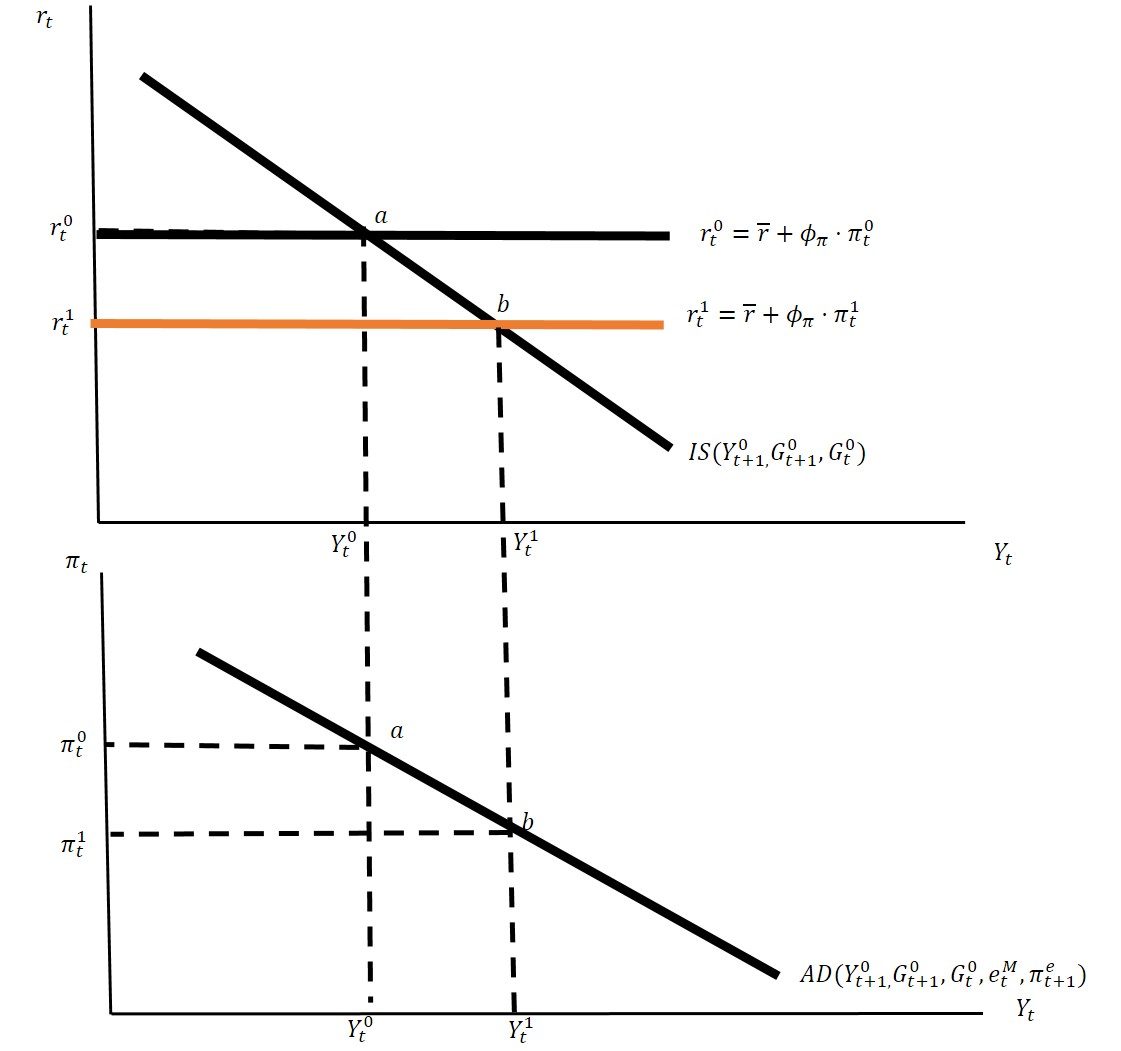
\includegraphics[width=\linewidth]{figAD0.jpg}
\end{column}
\begin{column}{0.38\textwidth}
\small
\begin{itemize}
\item Fix nominal money supply $M$.
\item Higher $P$ lowers real balances $M/P$.
\item Lower $M/P$ shifts LM left $\Rightarrow$ interest rate rises.
\item Higher interest rate reduces spending $\Rightarrow$ lower $Y$.
\end{itemize}
\end{column}
\end{columns}
\end{frame}

%------------------------------------------------
\begin{frame}{A simple IS--LM system (linear)}
\small
\begin{itemize}
\item \textbf{IS (goods market):} output falls when the real rate rises
\[
Y = \bar{A} - a r,\qquad a>0,
\]
where $\bar{A}$ summarizes autonomous spending (preferences, $G$, taxes, etc.).
\item \textbf{LM (money market):}
\[
\frac{M}{P} = kY - hi,\qquad k,h>0.
\]
\item \textbf{Fisher (in the background):} $i = r + \pi^e$.\ \ (For now take $\pi^e$ as given.)
\end{itemize}
\end{frame}

%------------------------------------------------
\begin{frame}{Solve IS + LM for $Y(P)$ (the AD equation)}
\small
From LM: $i = \frac{k}{h}Y - \frac{1}{h}\frac{M}{P}$, so
\[
r = i - \pi^e = \frac{k}{h}Y - \frac{1}{h}\frac{M}{P} - \pi^e.
\]
Plug into IS: $Y = \bar{A} - a r$,
\begin{align*}
Y &= \bar{A} - a\left(\frac{k}{h}Y - \frac{1}{h}\frac{M}{P} - \pi^e\right)\\[3pt]
\left(1 + a\frac{k}{h}\right)Y
&= \bar{A} + a\pi^e + \frac{a}{h}\frac{M}{P}.
\end{align*}

\vspace{0.3em}
\begin{itemize}
\item Therefore $Y$ increases in real balances $M/P$ and decreases in $P$.
\item This is the \textbf{downward slope of AD} in $(P,Y)$ space.
\end{itemize}
\end{frame}

%------------------------------------------------
\begin{frame}{What shifts AD (in equations)}
\begin{itemize}
\item AD is summarized by
\[
Y(P)=\frac{\bar{A}+a\pi^e+\frac{a}{h}\frac{M}{P}}{1+a\frac{k}{h}}.
\]
\item \textbf{AD shifts right} when, at each $P$, equilibrium $Y$ rises:
\begin{itemize}
\item $\bar{A}\uparrow$ (e.g., $G\uparrow$, lower taxes, optimism about future income)
\item $M\uparrow$ (higher nominal money supply)
\item $\pi^e\uparrow$ (given $i$, lower real rate; in the IS--LM derivation it enters through Fisher)
\end{itemize}
\end{itemize}
\end{frame}

%------------------------------------------------
\begin{frame}{Two textbook shifts (same as Lecture 3)}
\begin{columns}
\begin{column}{0.50\textwidth}
\centering
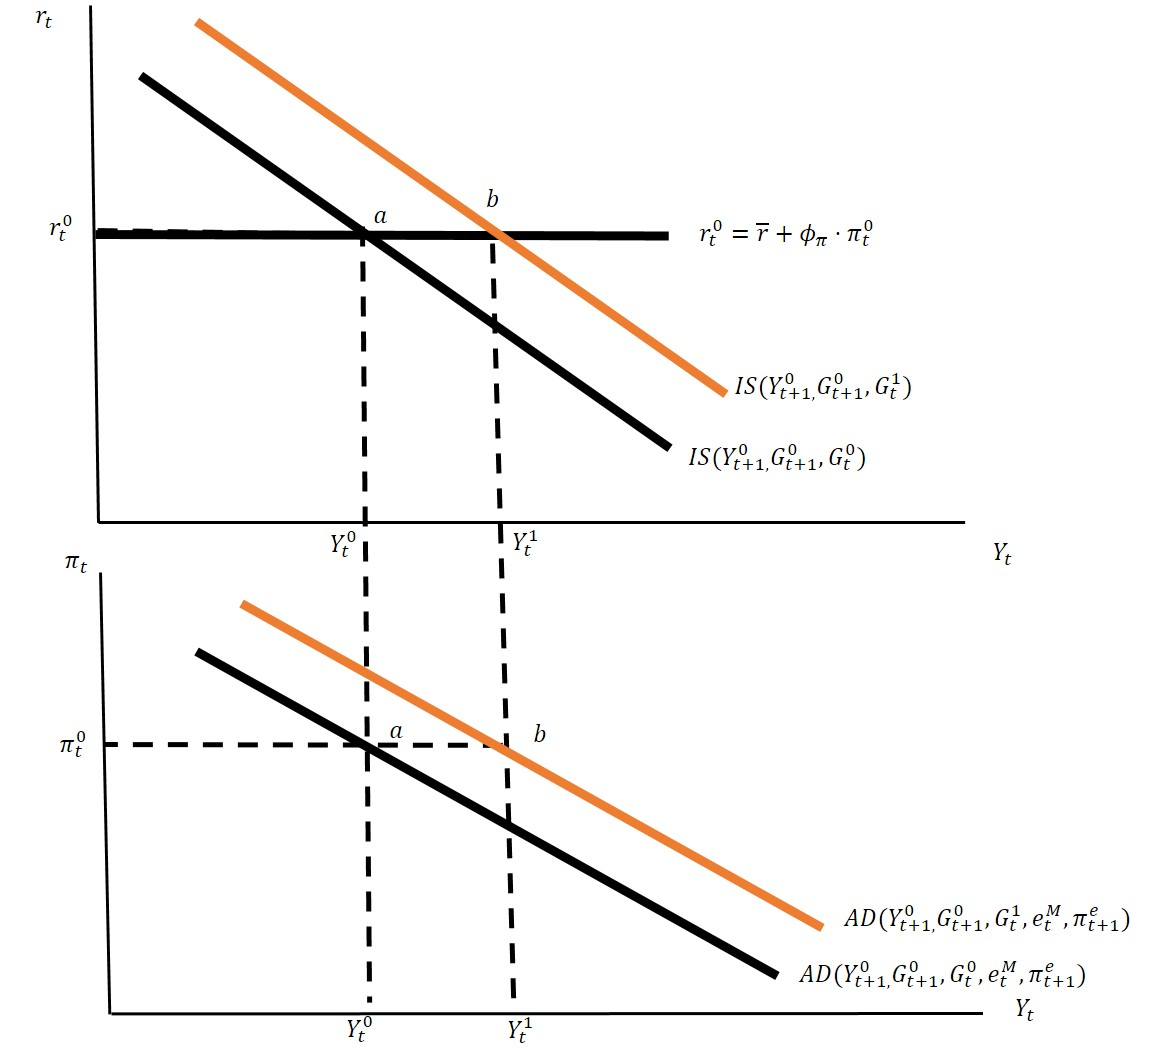
\includegraphics[width=\linewidth]{figAD1.jpg}\\[-2pt]
\small $G\uparrow$ (or $\bar{A}\uparrow$): AD shifts right
\end{column}
\begin{column}{0.50\textwidth}
\centering
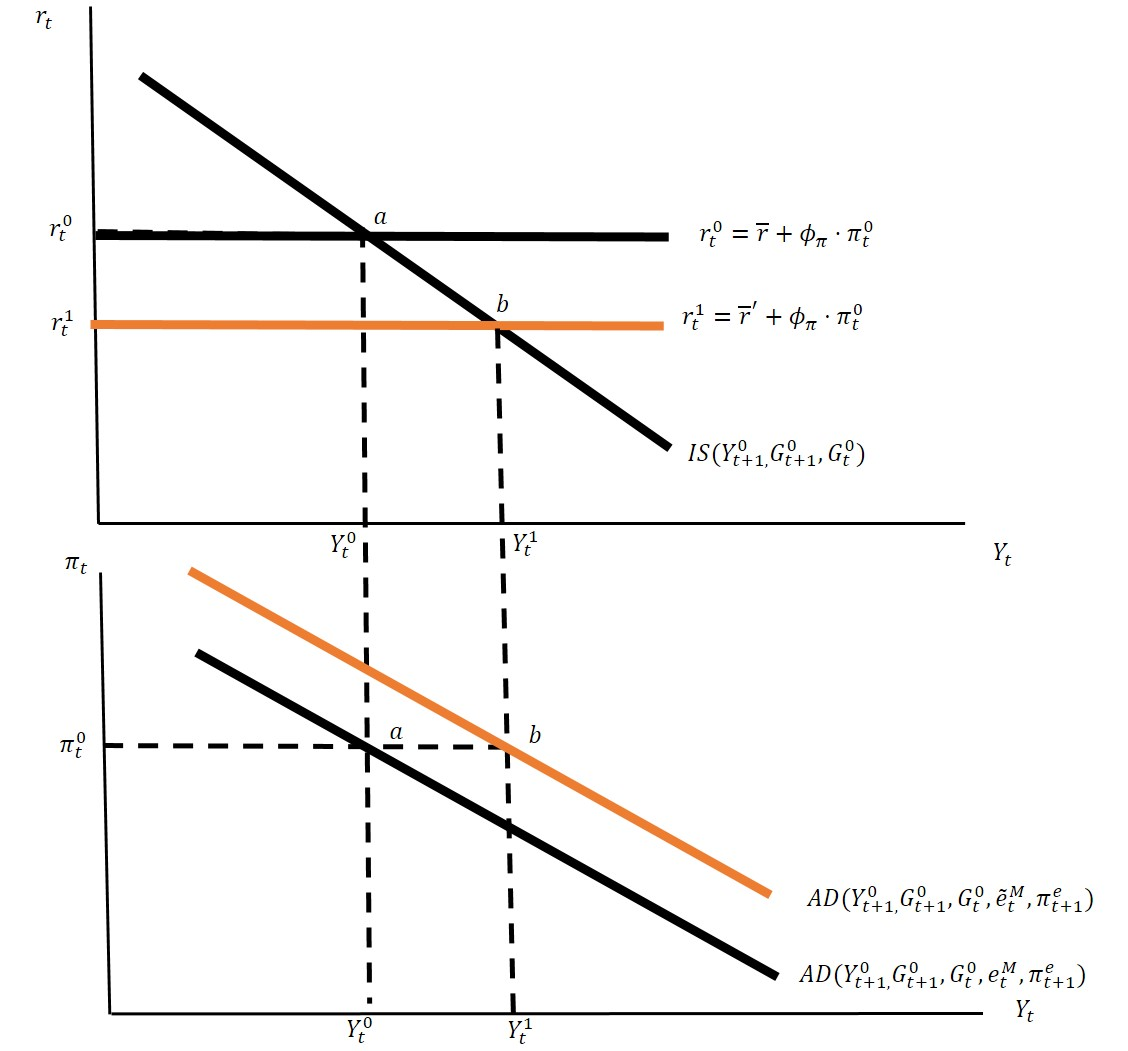
\includegraphics[width=\linewidth]{figAD2.jpg}\\[-2pt]
\small $M\uparrow$: real balances higher $\Rightarrow$ AD shifts right
\end{column}
\end{columns}
\end{frame}

%------------------------------------------------
\section{Aggregate supply in equations (SRAS + FE)}

%------------------------------------------------
\begin{frame}{FE as the long-run supply benchmark}
\begin{columns}
\begin{column}{0.62\textwidth}
\centering
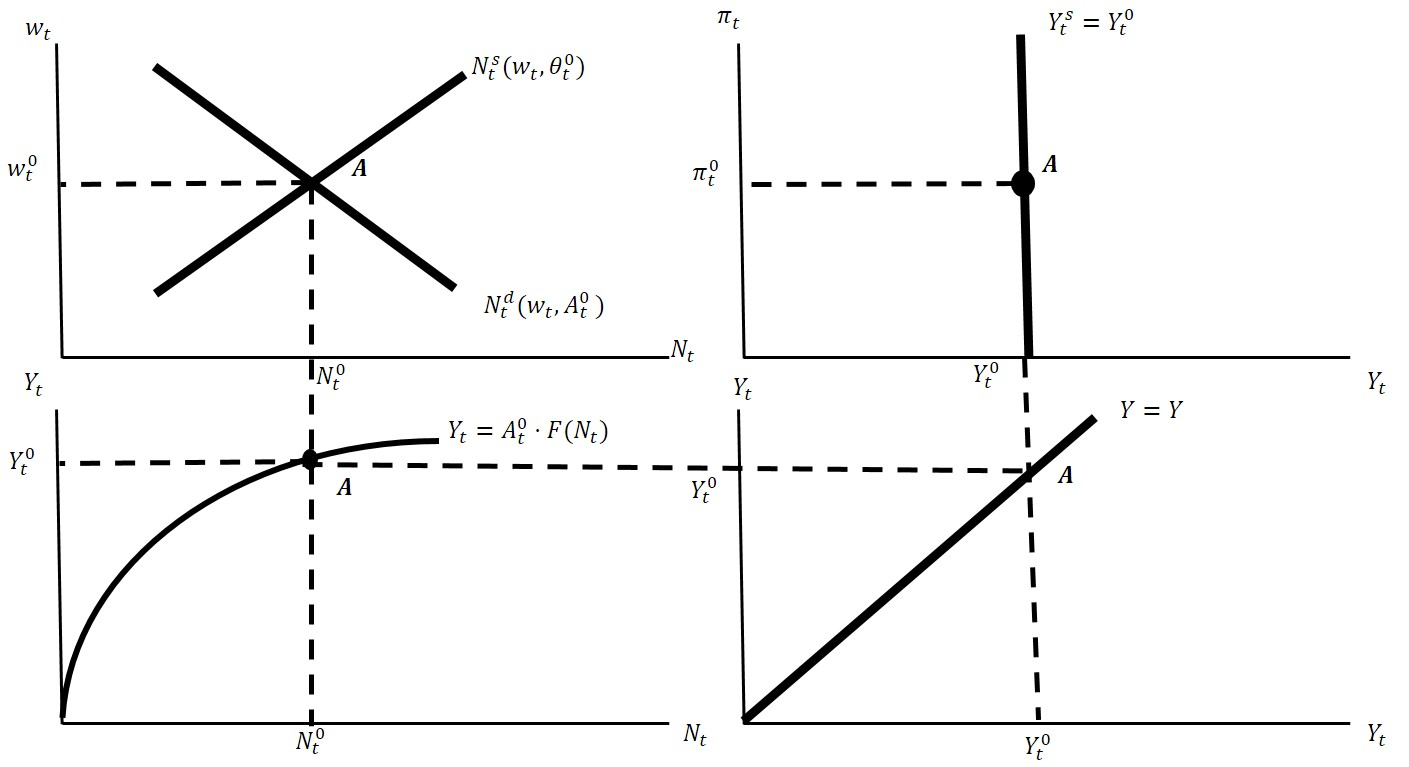
\includegraphics[width=\linewidth]{figAS0.jpg}
\end{column}
\begin{column}{0.38\textwidth}
\small
\begin{itemize}
\item FE output $Y^{FE}$ comes from the RBC supply block (labor market + production).
\item In the long run, prices adjust so output returns to $Y^{FE}$.
\item FE shifts with technology, factor supply, and capital.
\end{itemize}
\end{column}
\end{columns}
\end{frame}

%------------------------------------------------
\begin{frame}{SRAS as ``price surprises move output'' (level form)}
\small
A convenient reduced form (Lucas/expectations-augmented supply):
\[
y = y^{FE} + \alpha\,(p - p^e),\qquad \alpha>0.
\]
\begin{itemize}
\item If $p>p^e$ (prices higher than expected), real wages are lower than expected $\Rightarrow$ firms hire more $\Rightarrow$ output rises.
\item If $p<p^e$, output falls below $y^{FE}$.
\item The slope of SRAS in $(p,y)$ space is $1/\alpha$.
\end{itemize}
\end{frame}

%------------------------------------------------
\begin{frame}{SRAS written in output-gap notation}
\small
Define output gap $x \equiv y-y^{FE}$. Then
\[
x = \alpha\,(p - p^e).
\]
\begin{itemize}
\item Output gap is proportional to the \textbf{price-level surprise} $(p-p^e)$.
\item A left shift of AS in Lecture 3 corresponds to shocks that raise marginal cost for given $x$,
or (equivalently) raise the $p$ needed to produce a given $y$.
\end{itemize}

\vspace{0.3em}
\begin{itemize}
\item Next lecture we will rewrite this in inflation form and specify how $p^e$ evolves (expected inflation).
\end{itemize}
\end{frame}

%------------------------------------------------
\begin{frame}{Supply-side shifts in the figures}
\begin{columns}
\begin{column}{0.50\textwidth}
\centering
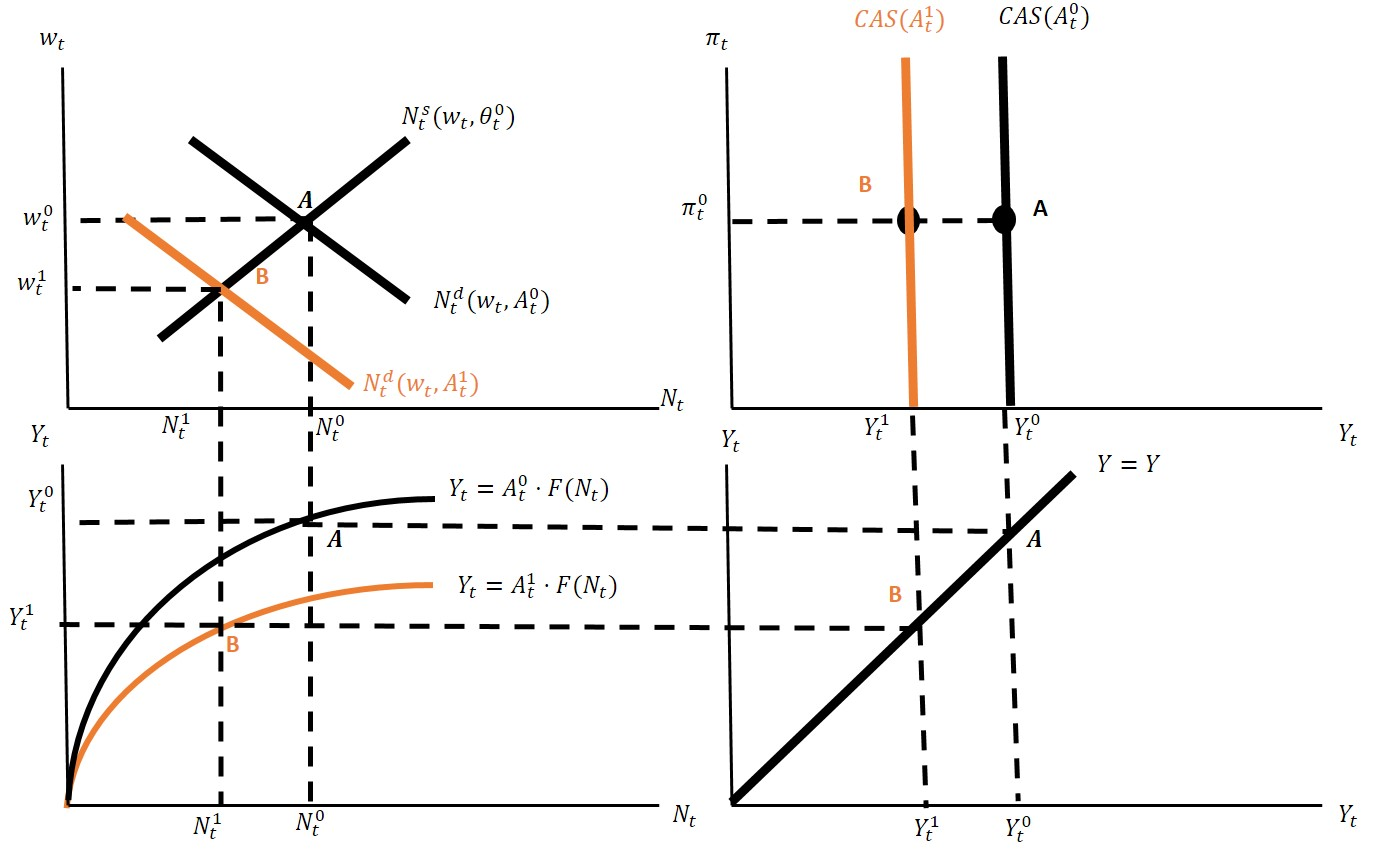
\includegraphics[width=\linewidth]{figAS1.jpg}\\[-2pt]
\small $A\downarrow$ shifts FE / CAS left
\end{column}
\begin{column}{0.50\textwidth}
\centering
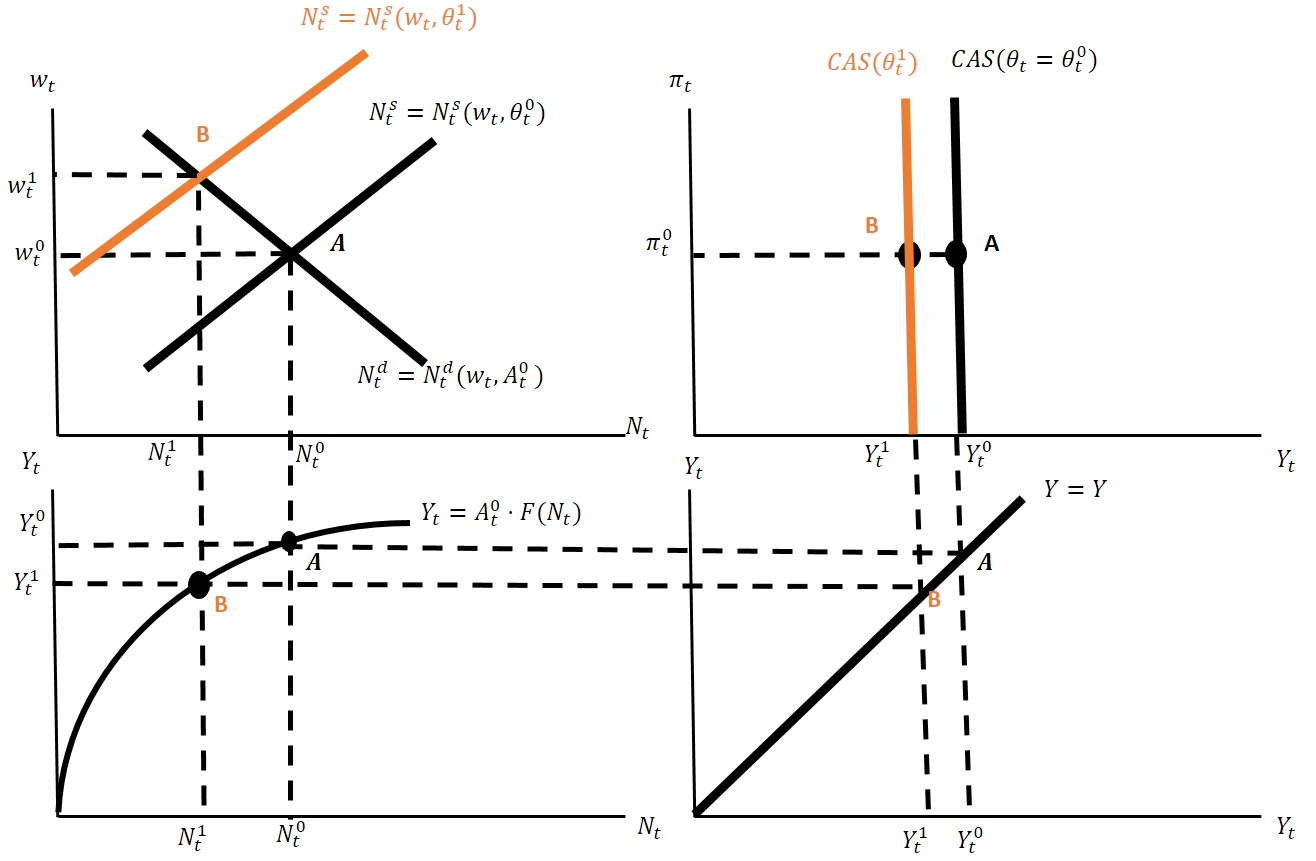
\includegraphics[width=\linewidth]{figAS2.jpg}\\[-2pt]
\small labor supply $\downarrow$ shifts FE / CAS left
\end{column}
\end{columns}
\end{frame}

%------------------------------------------------
\section{Equilibrium and comparative statics}

%------------------------------------------------
\begin{frame}{AD--AS equilibrium (in one picture)}
\centering
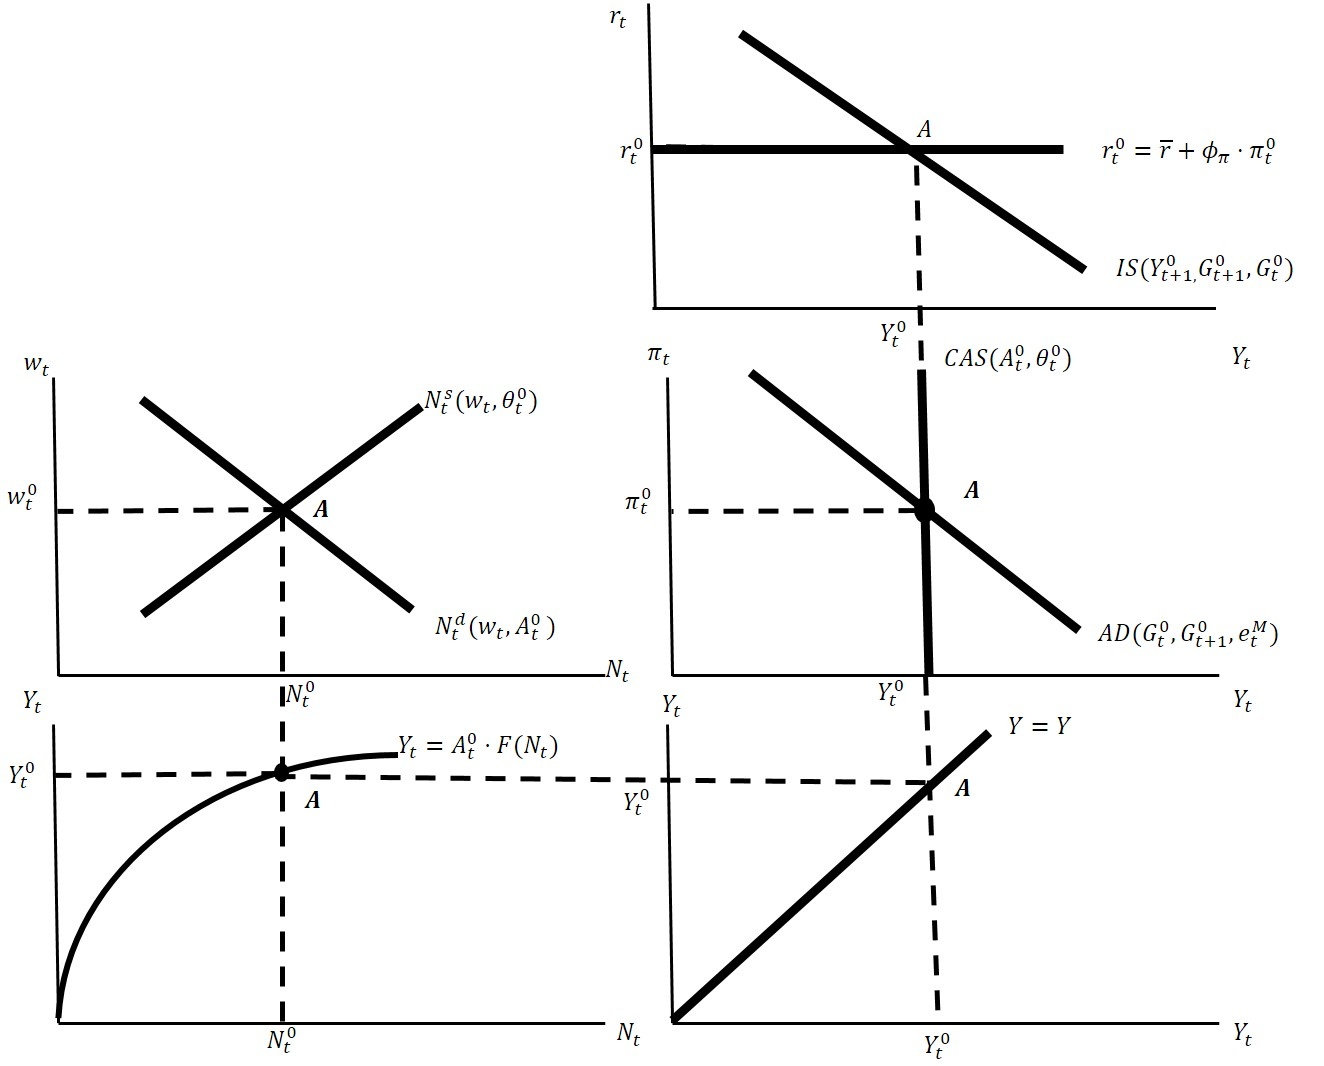
\includegraphics[width=0.90\linewidth]{figADAS.jpg}
\end{frame}

%------------------------------------------------
\begin{frame}{AD--AS equilibrium (solve once)}
\small
Use a simple AD reduced form $y = \bar{y}_D - \phi\,p$ with $\phi>0$ (downward slope), and SRAS
$p = p^e + \lambda (y-y^{FE})$ with $\lambda>0$ (upward slope).

\vspace{0.2em}
\begin{itemize}
\item Substitute AD into SRAS:
\[
p = p^e + \lambda\big(\bar{y}_D - \phi p - y^{FE}\big).
\]
\item Solve for $p$:
\[
(1+\lambda\phi)p = p^e + \lambda(\bar{y}_D - y^{FE})
\quad\Rightarrow\quad
p = \frac{p^e + \lambda(\bar{y}_D - y^{FE})}{1+\lambda\phi}.
\]
\item Then $y$ follows from AD: $y=\bar{y}_D-\phi p$.
\end{itemize}
\end{frame}

%------------------------------------------------
\begin{frame}{Demand expansion: why $(Y,P)$ move together}
\begin{columns}
\begin{column}{0.62\textwidth}
\centering
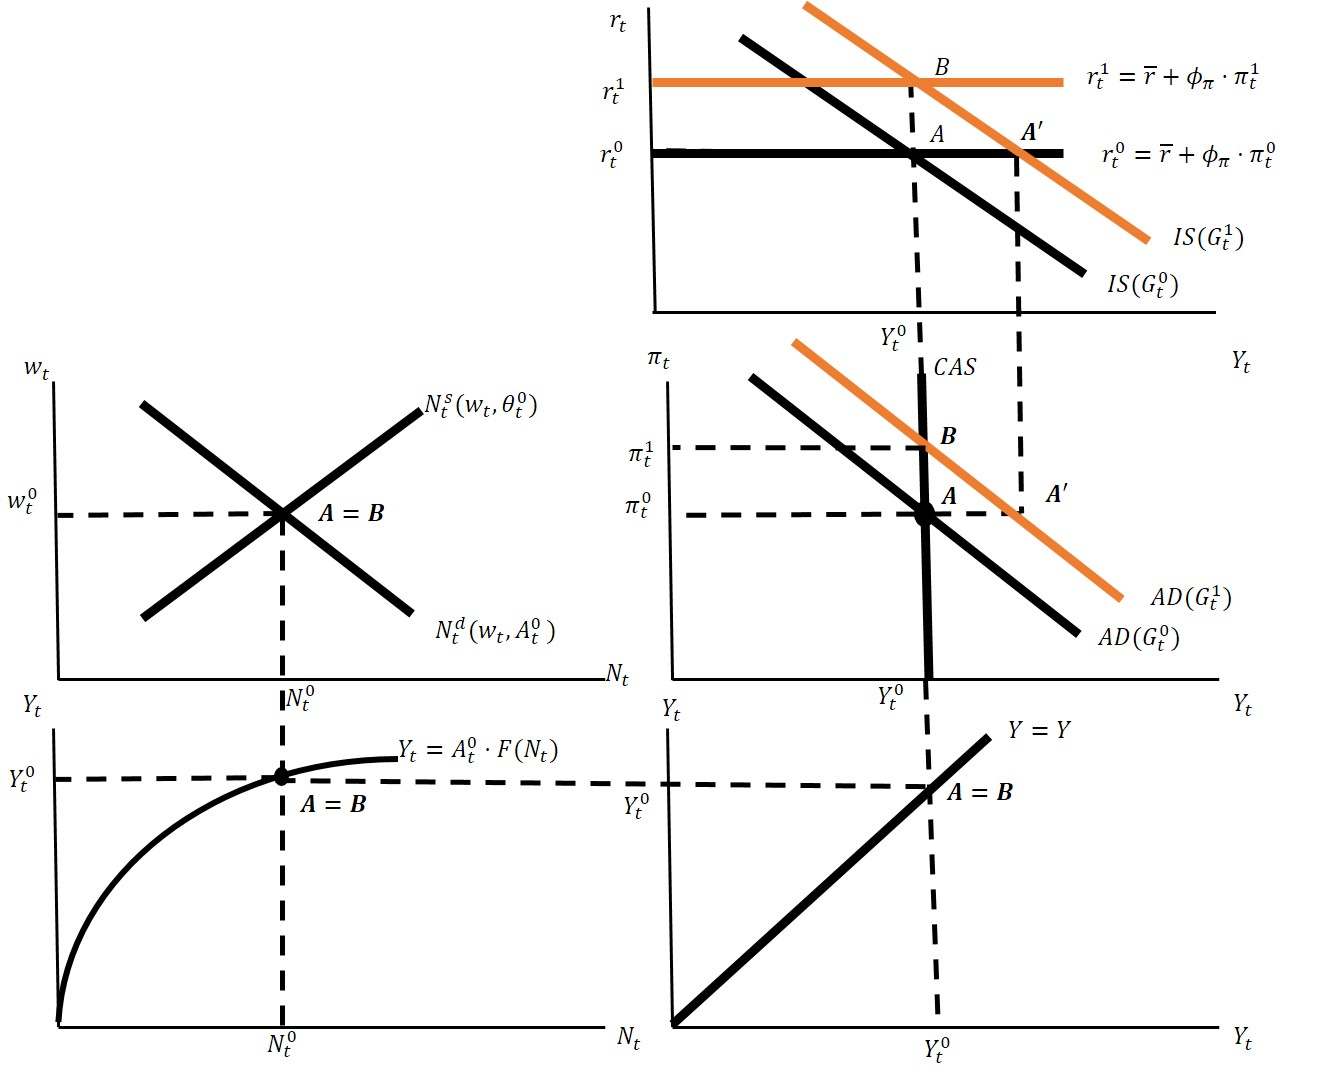
\includegraphics[width=\linewidth]{figADAS1.jpg}
\end{column}
\begin{column}{0.38\textwidth}
\small
\begin{itemize}
\item Demand expansion means $\bar{y}_D\uparrow$ (AD shifts right).
\item From the solved expression: $p$ rises when $\bar{y}_D$ rises.
\item AD then implies $y$ rises as well.
\end{itemize}
\end{column}
\end{columns}
\end{frame}

%------------------------------------------------
\begin{frame}{Monetary easing: one parameter shift, same logic}
\begin{columns}
\begin{column}{0.62\textwidth}
\centering
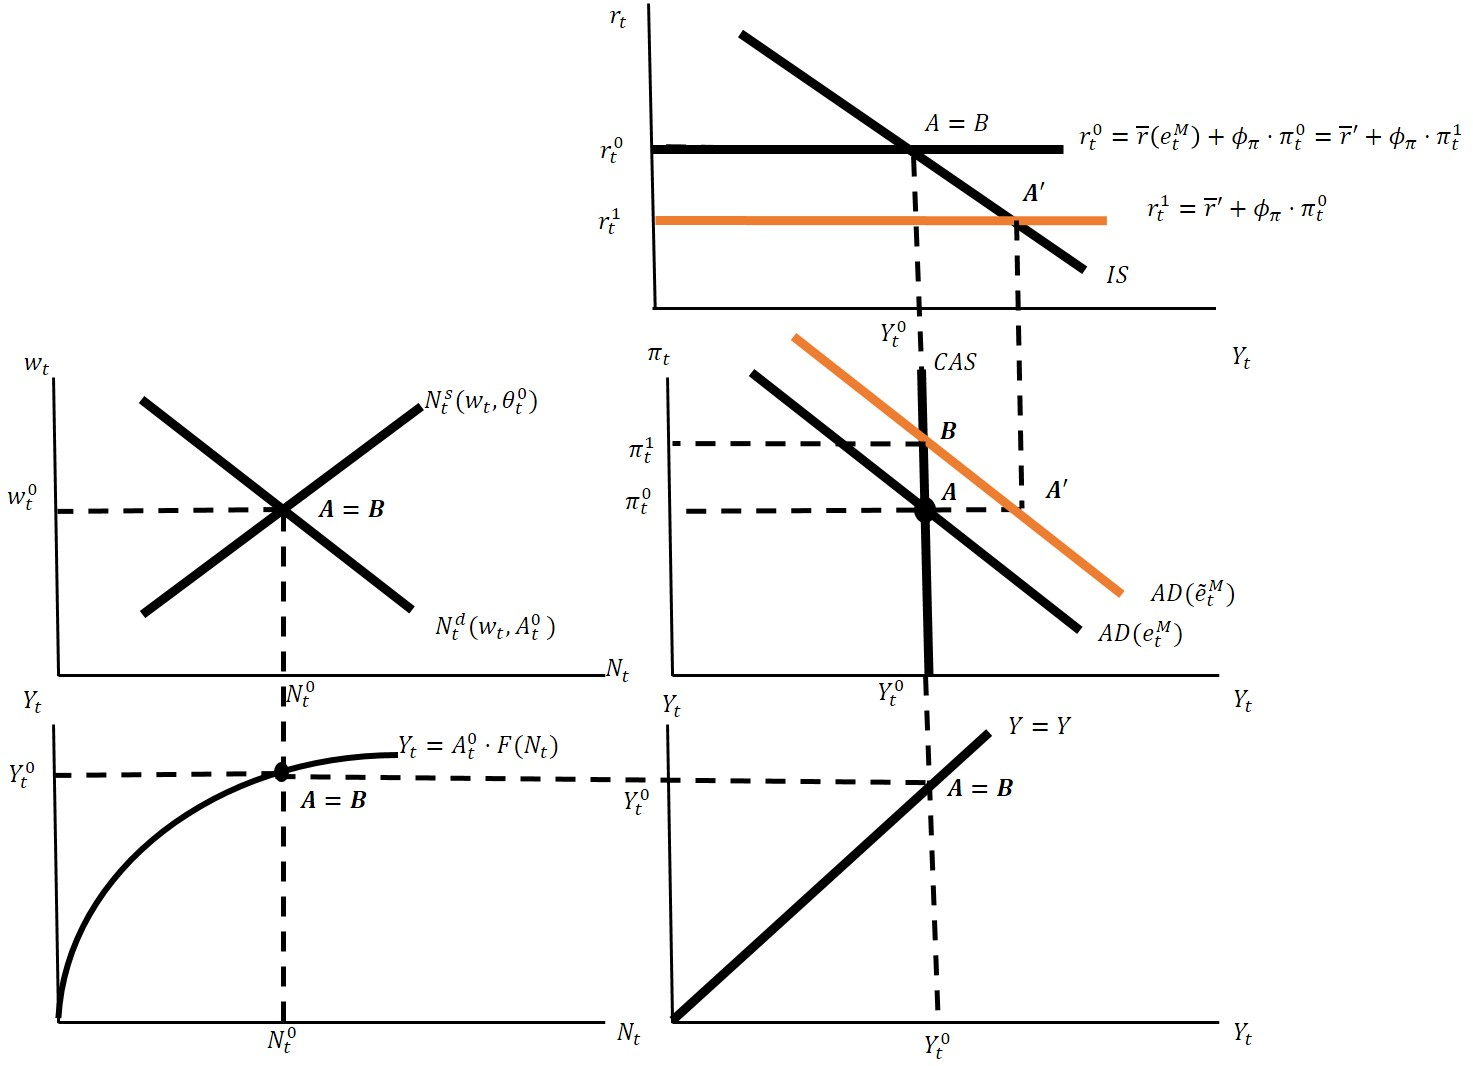
\includegraphics[width=\linewidth]{figADAS2.jpg}
\end{column}
\begin{column}{0.38\textwidth}
\small
\begin{itemize}
\item Monetary easing shifts AD right (for each $P$, higher $Y$).
\item In the IS--LM derivation, this is $M\uparrow$ or lower $i$ (higher real balances / lower real rate).
\item Equilibrium: $(Y,P)$ rise together in the short run.
\end{itemize}
\end{column}
\end{columns}
\end{frame}

%------------------------------------------------
\begin{frame}{Supply contraction: stagflation in one line}
\begin{columns}
\begin{column}{0.62\textwidth}
\centering
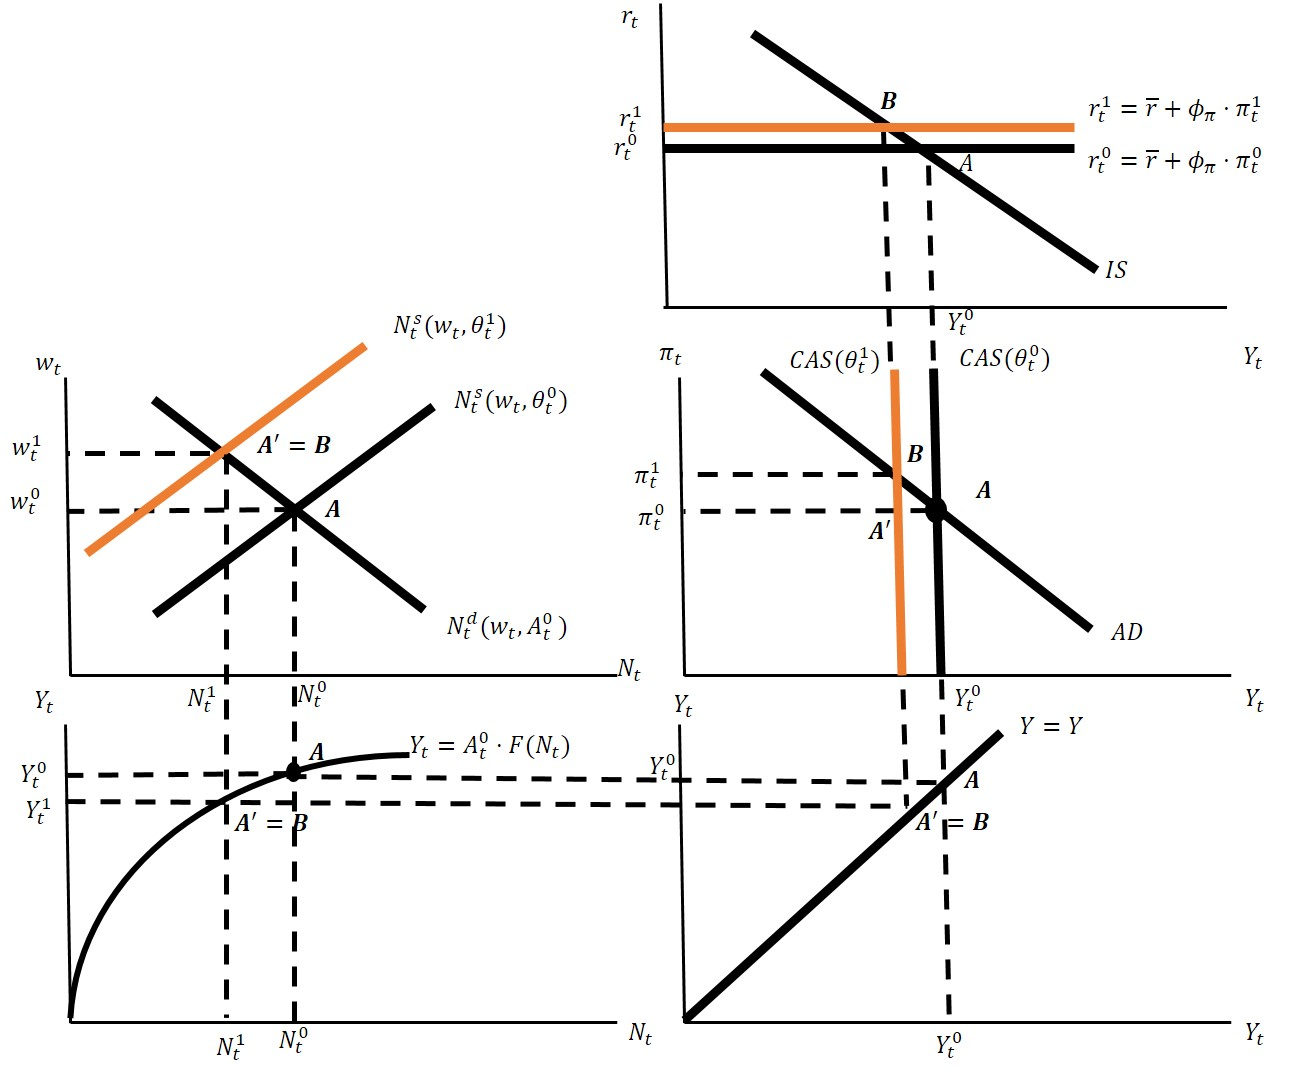
\includegraphics[width=\linewidth]{figADAS3.jpg}
\end{column}
\begin{column}{0.38\textwidth}
\small
\begin{itemize}
\item Supply contraction means $y^{FE}\downarrow$ or AS shifts up/left.
\item In the solved expression: if $y^{FE}$ falls, $p$ rises.
\item But lower $y^{FE}$ also pushes output down.
\end{itemize}
\end{column}
\end{columns}
\end{frame}

%------------------------------------------------
\begin{frame}{Medium run: expected price level catches up}
\begin{columns}
\begin{column}{0.62\textwidth}
\centering
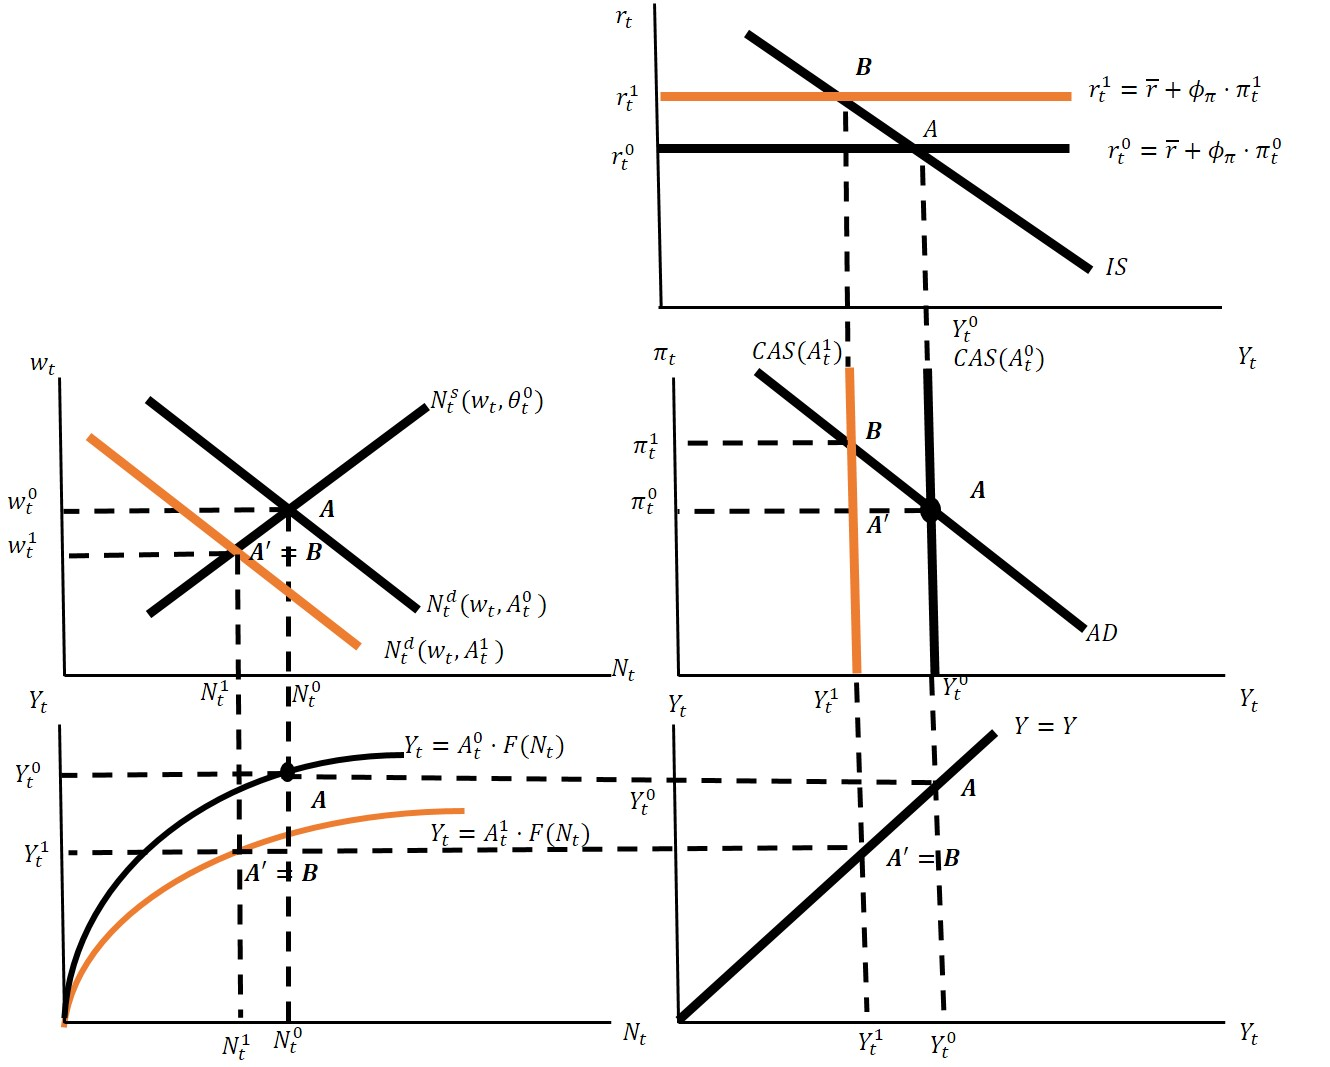
\includegraphics[width=\linewidth]{figADAS4.jpg}
\end{column}
\begin{column}{0.38\textwidth}
\small
\begin{itemize}
\item SRAS depends on $p^e$. When $p^e$ updates, SRAS shifts.
\item Medium-run logic: $p^e \uparrow$ until output returns to $y^{FE}$.
\item This is the bridge to next lecture: specify how $p^e$ evolves $\Rightarrow$ expected inflation.
\end{itemize}
\end{column}
\end{columns}
\end{frame}

%------------------------------------------------
\section{One-page summary}

%------------------------------------------------
\begin{frame}{Cheat sheet: what each symbol means in the math AD--AS}
\small
\begin{itemize}
\item \textbf{Demand side (AD):} $y=\bar{y}_D-\phi p$ \quad (downward in $p$)
\begin{itemize}
\item $\bar{y}_D$ collects \emph{demand shifters}: $G$, taxes, wealth/optimism, monetary stance ($M$, $i$), etc.
\end{itemize}
\item \textbf{Supply side (SRAS):} $p=p^e+\lambda(y-y^{FE})$ \quad (upward in $y$)
\begin{itemize}
\item $y^{FE}$ is potential output from the RBC supply block (technology, labor, capital).
\item $p^e$ is the expected price level; updating $p^e$ shifts SRAS over time.
\end{itemize}
\item \textbf{Unemployment link:} $u-u^n\approx-\gamma x$ \quad (Okun).
\end{itemize}
\end{frame}

%------------------------------------------------
\begin{frame}{Next lecture (without naming ``Old Keynesian'' yet)}
\begin{itemize}
\item Replace $p^e$ with a rule for expected inflation (how expectations are formed).
\item Replace the level-form SRAS with an inflation form (Phillips curve language).
\item Introduce central bank practice: inflation targeting, Taylor rules, and how a policy rule shifts AD.
\end{itemize}
\end{frame}

\end{document}
